\chapter{ОБЗОР ЛИТЕРАТУРЫ}\label{chap1}

%Первая глава всегда посвящена обзору литературы. В начале каждой главы необходимо написать небольшую аннотацию о содержании главы (так называемая \textit{врезка}). Например:

В настоящей глава формулируются основные понятия и определения, используемые в курсовой работе.Приводится классификация (согласно работе \cite{GabasovKirillovaPU}) принципов управления, используемых в современной теории управления. Объясняется принцип управления в режиме реального времени в применении к реализации оптимальных обратных связей в задачах оптимального управления с конечным горизонтом планирования \cite{GabasovDmitrukKirillova15a}.


%%%%%%%%%%%%%%%%%%%%%%%%%%%%%%%%%%%%%%%%%%%%%%%%%%%%%%%%%%%%%%%%%%%%%%%%%%%%%%%%
\section{Задачи оптимального управления}\label{1sec:optimal-control}
Человек занимается управлением на протяжении всей своей жизни для обеспечения желаемого течения тех или иных процессов или сам предпринимает необходимые действия и принимает соответсвующее решения.

Теория оптимального управления,отражающая современный этап развития вариационного исчилсения,возникла в середине \RNumb{20} века в связи с задачами, поставленными практикой в различных областях развития новой техники.

Существует два взгляда на теорию оптимального управления.Согласно одному из них,теория оптимального управления — раздел современного вариационного исчисления.В соответствии с этим взглядом дадим следующее определние.
Управления — элементы функциональных пространств, по которым ищется экстремум выбранного функционала качества.
Главной задачей данной теории является анализ решения экстремальной задачи (существование, единственность, непрерывная зависимость решений, необходимые и достаточные условия оптимальности).

Другой взгяд трактует данную теорию как раздел современной теории управления, представляющей естественное развитие классической теории управления.
В этом случае выделим следующее определения для управления.
 Управления — это процесс, в котором для достижения нужного поведения объекта управления в каждый текущий момент времени создаются целенаправленные(управляющие) воздействия на объект управления в зависимотси от доступной к этому моменту информации о поведении объекта и действующих на него возмущений.

%%%%%%%%%%%%%%%%%%%%%%%%%%%%%%%%%%%%%%%%%%%%%%%%%%%%%%%%%%%%%%%%%%%%%%%%%%%%%%%%
\section{Программные и позиционные решения}\label{1sec:Solution}

При управлении динамическим объектом используются три принципа: управление по разомкнутому контуру (программное управление), управление по замкнутому контуру (позиционное управление), управление в реальном времени.

\begin{figure}[h]

\centering

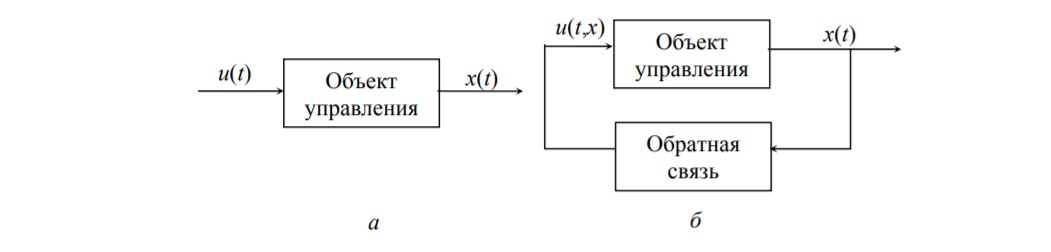
\includegraphics[width=\linewidth]{image1.jpg}

\caption{а) разомкнутый контур; б) замкнутый контур}

\label{fig:mpr}

\end{figure}

\begin{definition} 
Программное управление — управление, при котором (программные) управляющие воздействия (программы) планируются по априорной информации до начала процесса управления и не корректируются в процессе управления. 
\end{definition}

Программное управление редко применяется на практике, поскольку не учитывает неточности математического моделирования физических систем и возмущения, косвенная информация о которых доступна, как правило, в процессе управления. Фундаметом этого метода является принцип максимума Понтрягина. 

\begin{definition} 
Позиционное управление — управление, при котором (позиционные) управляющие воздействия создаются в процессе управления по текущим позициям, которые аккумулируют информацию, доступную к текущему моменту.
\end{definition}

%Динамическое программиирование является одним из основных методов реализации позиционного управления.

\begin{definition} 
Cинтез оптимальных систем управления — построение оптимальных позиционных управляющих воздействий.
\end{definition}
При создании систем по принципу замкнутого контура используются связи трех типов:\emph{прямые}, \emph{обратные} и \emph{комбинированные} (рис. 1.2).
\begin{figure}[h]

\centering

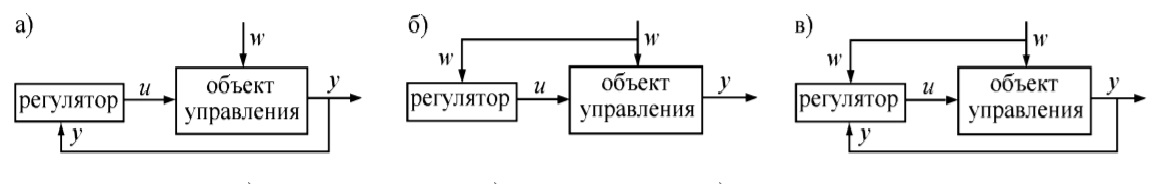
\includegraphics[width=\linewidth]{image2.jpg}

\caption{а) обратная связь; б) прямая связь; в) комбинированная связь}

\label{fig:mpr}

\end{figure}

 Связь называется прямой, если она преобразует в управляющее воздействие доступную информацию о наблюдаемых входных сигналах. Обратная связь по состоянию преобразует в управляющее воздействие информацию о состоянии объекта. В комбинированной связи преобразуется информация обоих типов.
 
 Для позиционного управления характерна следующая особенность. Проблема синтеза в рамках принципа управления по замкнутому контуру не удается решить из-за проклятия размерности ни с помощью принципа максимума, ни с помощью динамического программирования Беллмана. 
 
 Решение данной проблемы состоит в переходе к современному принципу управления — оптимальному управлению в реальном времени. При управлении динамическим объектом в реальном времени связи не строятся, а необходимые для управления их текущие значения формируются в реальном времени по ходу каждого конкретного процесса.
 


%%%%%%%%%%%%%%%%%%%%%%%%%%%%%%%%%%%%%%%%%%%%%%%%%%%%%%%%%%%%%%%%%%%%%%%%%%%%%%%%

\section{Реализация оптимальных обратных связей в реальном времени}\label{1sec:Feedback}
Принцип управления в реальном времени и подход к реализации оптимоной обратной связи в реальном времени опишем на примере следующей задачи оптимального управления.

\begin{equation} \label{1problem}
    c^Tx(t_f)\to \min,
    \end{equation}
$$
    \dot{x}=A(t)x+B(t)u,\quad x(t_0)=x_0^*,
    $$
$$
    x(t_f) \in X_f,\quad  u(t)\in U, \quad  t\in T = [t_*, t^*],
    $$
где  $x = x(t)\in \mathbb{R}^n$ — состояение модели управления в момент времени t,
$u = u(t)\in \mathbb{R}^r$ — значение управляющего воздействия в момент t, 
$A(t)\in \mathbb{R}^{n\times n}$,
$B(t)\in \mathbb{R}^{n\times r}$,
$x_0^*$ — известное начальное состояние объекта.
$X_f=\{x\in \mathbb{R}^n: g_*\leq Hx \leq g^*\}$ --- терминальное
множество, $H\in \mathbb{R}^{m\times n}$, $g_*,$ $g^* \in \mathbb{R}^m$;
$U=\{u\in \mathbb{R}^r: u_*\le u\le u^*\}$ --- множество доступных значений
управляющего воздействия.

\begin{definition}  Управляющее воздействие $u(t)\in U$, $t\in T$, называется программой, если соответствующая ему
траектория $x(t)$, $t\in T$, математической модели (\ref{1problem}) удовлетворяет
условию $x(t_f)\in X_f$.
\end{definition}

\begin{definition}  Программа $u^0(t)$, $t\in T$,
называется оптимальной (программным решением задачи (\ref{1problem})), если на соответствующей ей (оптимальной) траектории $x^0(t)$, $t\in T$, выполняется равенство $c^Tx^0(t_f) = \min_u c^Tx(t_f),$ где минимум ищется среди всех программ. 
\end{definition}
%%%%%%%%%%%%%%%%%%%%%%%%%%%%%%%%%%%%%%%%%%%%%%%%%%%%%%%%%%%%%%%%%%%%%%%%%%%%%%%%

Задача (\ref{1problem})) рассматривается в классе диксретных управляющих воздействий:

$u\equiv u(\tau), t\in [ \tau,\tau + h[, \tau = T_h = \{t_*,t_* + h,...,t^* - h\} (h = (t^* - t_*)/N, N > 0),$.

Чтобы ввести понятие классической оптимальной обратной связи, погрузим задачу (\ref{1problem}) в семейство задач

\begin{equation} \label{2problem}
    c^Tx(t_f)\to \min,
    \end{equation}
$$
    \dot{x}=A(t)x+B(t)u,\quad  x(\tau) = z,
    $$
$$
    x(t_f) \in X_f,\quad  u(t)\in U, \quad  t\in T(\tau) = [\tau, t^*],
    $$
    
Пусть $u^0(t|\tau,z),\quad t\in T(\tau),$ — оптимальная программа задачи (\ref{2problem})) для позиции ($\tau$,z).

Функция
\begin{equation} \label{3problem}
    u^0(\tau,z) = u^0(\tau|\tau,z),\quad z\in X_\tau,\quad \tau \in T_h,
    \end{equation}
называется оптимальной обратной связью (позиционным решением задачи (\ref{1problem})).

Оптимальная обратная связь (\ref{3problem}) предназначена для управления физическим объектом. Замкнем ею объект управления и запишем поведение замкнутой системы в форме
\begin{equation} \label{4problem}
\dot{x}=A(t)x+B(t)u^0(t,x),\ x(t_*) = x_0,
 \end{equation}
где $u^0(t,x) = u^0(t,x(t))\equp u^0(\tau,x(\tau)),\quad t\in [\tau,\tau + h[,\quad \tau\in T_h$.

Рассмотрим поведение систымы (\ref{4problem}) в конкретном процессе управления.
$$\dot{x^*(t)}=A(t)x^*(t)+B(t)u^0(t,x^*(t)),\quad x^*(t_*) = x_0,$$
$$u^*(t)\equiv u^0(\tau,x^*(\tau)) = u^0(\tau|\tau,x^*(\tau)),\quad t\in[\tau,\tau + h[,\quad  \tau \in T_h,$$

Функцию $u^*(t), t\in T$ будем называть реализацие опитмальной обратной связи (\ref{3problem}) в конкретном процессе управления. 


Перейдём к описанию принципа оптимального управления в реальном времени, при котором обратная связь  (\ref{3problem}) не строится,а при каждом $\tau \in T_h$ текущее управляющее воздействие $u^*(\tau)$ создаётся в процессе управления для текущей позиции $(\tau,x^*(\tau))$.

Пусть  $\delta(\tau)$ — время вычисления значения $u^*(\tau), \tau \in T_h$
\begin{definition}
Устройтво,способное вычислять значение $u^*(\tau), \tau \in T_h$ за время $\delta(\tau)$ < h,называется оптимальным регулятором, реализующим оптимальную обратную свзять (\ref{3problem}) в реальном времени.
\end{definition}

Из определия оптимальной обратной связи, оптимальный регулятрор в каждый момент времени $\tau \in T_h$ должен решить задачу

\begin{equation} \label{5problem}
    c^Tx(t_f)\to \min,
    \end{equation}
$$
    \dot{x}=A(t)x+B(t)u,\quad x(\tau) = x^*(\tau),
    $$
$$
    x(t_f) \in X_f,\quad  u(t)\in U, \quad  t\in T(\tau).
    $$
    
Запишем формулу Коши для линейной системы.

$$x(t^*) = F(t^*,\tau)x^*(\tau) + \int_{\tau}^{t^*} F(t^*,t)B(t)u(t)\,dt $$
где $F(t^*,t)$ — фундаментальная матрица.
\begin{equation} \label{7problem}
x(t^*) = F(t^*,\tau)x^*(\tau) +  \sum_{s=\tau}^{t^*-h}\int_{s}^{s+h} F(t^*,t)B(t)\,dt   u(s)
\end{equation}
Преобразуем равенство умножив (\ref{7problem}) на матрицу H.

\begin{equation} \label{8problem}
Hx(t^*) = HF(t^*,\tau)x^*(\tau) +  \sum_{s=\tau}^{t^*-h}\int_{s}^{s+h} HF(t^*,t)B(t)\,dt   u(s)
\end{equation}

Равенство  (\ref{8problem}) эквивалетно следующему:

$$Hx(t^*) = \Phi(\tau)x^*(\tau) +  \sum_{s=\tau}^{t^*-h}D(s)u(s)$$

где

$$\Phi(t) = HF(t^*,t) \quad \Phi(t^*) = H, \quad \dot{\Phi} = -\Phi A(t);$$
$$D(s) =\int_{s}^{s+h} \Phi(t)B(t)\,dt,\quad s\in T_h $$ 

Таким образом,исходная задача (\ref{5problem}) эквивалентна следующей задаче линейного программирования:

\begin{equation} \label{9problem}
\sum_{t\in T_h(\tau)}^{}c'(t)u(t) \to \min,\quad  g_*(\tau) \leq \sum_{s\in T_h(\tau)}^{}D(s)u(s) \leq g^*(\tau),
\end{equation}
$$ u_*\leq u(t) \leq u^*,\quad t \in T_h(\tau)$$

где
$$c'(t) = \int_{s}^{s+h} F(t^*,t)B(t)\,dt,\quad s\in T_h,\quad \dot F(t^*,t) = - F(t^*,t)A(t),\quad F(t^*,t^*) = c;$$

$$g_*(\tau) = g_* - \Phi(\tau)x^*(\tau),\quad g^* - \Phi(\tau)x^*(\tau);$$



В настоящей глава были рассмотрены основные понятия и определения.Была получена классификация принципов управления, используемых в современной теории управления. Рассмотрен принцип управления в режиме реального времени в применении к реализации оптимальных обратных связей в задачах оптимального управления с конечным горизонтом планирования.

\bigskip